\documentclass[3p,11pt]{elsarticle}

% --- PAQUETES OPTIMIZADOS PARA ELSARTICLE ---
\usepackage[utf8]{inputenc}
\usepackage[spanish]{babel}
\usepackage{amsmath}
\usepackage{graphicx}
\usepackage{booktabs}
\usepackage{natbib}
\usepackage{floatrow}
\usepackage{lineno}
\usepackage{hyperref}
\usepackage{siunitx}


\graphicspath{{figures/}}

\floatsetup[figure]{capposition=top}


% --- CONFIGURACIÓN DE FORMATO DE PÁRRAFOS ---
\setlength{\parindent}{0pt}        
\setlength{\parskip}{6pt}          

% --- CONFIGURACIÓN DE CITAS ---
\bibliographystyle{elsarticle-harv}

\begin{document}

\begin{frontmatter}

\title{Análisis de Vulnerabilidad Externa para economías iberoamericanas: Una Aplicación del Modelo VECM}

\author[inst1]{Manuel Alejandro Hidalgo Pérez}
\address[inst1]{Departamento de Economía, Universidad Pablo de Olavide, Sevilla, España}

\begin{abstract}
Este documento desarrolla un indicador econométrico de vulnerabilidad externa para economías iberoamericanas mediante un Modelo de Vectores de Corrección de Errores (VECM). La metodología extiende el marco de Izquierdo, Romero y Talvi (2008) mediante: construcción de un indicador sintético, optimización endógena de pesos, y validación estadística de capacidad predictiva.

El modelo estima relaciones de cointegración entre el PIB y variables externas clave (términos de intercambio, producción del G7, condiciones financieras globales), extrayendo el Término de Corrección de Error como base para un indicador compuesto que integra desequilibrios de largo plazo y volatilidad de corto plazo. La velocidad de corrección se estima en 25\% trimestral, y los pesos óptimos mejoran la correlación predictiva en 24.4\% respecto a pesos equiponderados.

Los resultados (2000-2024, 99 observaciones) demuestran capacidad predictiva estadísticamente significativa, con correlación negativa de -0.196 entre vulnerabilidad actual y crecimiento futuro del PIB. El indicador identifica correctamente los principales episodios de estrés: crisis 2002-2003, 2008-2009, 2012-2015, y 2020-2021.
\end{abstract}

\begin{keyword}
Vulnerabilidad externa, VECM, Cointegración, Alerta temprana, Indicador sintético, Optimización predictiva
\MSC[2010] 00-01, 99-00
\JEL  C32, F34, F47, O54
\end{keyword}

\end{frontmatter}

\section{Introducción}

Las economías latinoamericanas exportadoras de materias primas enfrentan una exposición estructural a la volatilidad del entorno económico global. Las fluctuaciones en los precios de commodities, los cambios en las condiciones financieras internacionales, las variaciones en la demanda de los principales socios comerciales y los movimientos en los flujos de capital pueden generar shocks externos de magnitud considerable, con profundas repercusiones sobre el crecimiento económico, la estabilidad macroeconómica y la sostenibilidad fiscal. En este contexto, el desarrollo de herramientas robustas y oportunas para el monitoreo y la predicción de episodios de vulnerabilidad externa constituye una prioridad fundamental para la formulación de políticas macroeconómicas efectivas y la gestión proactiva del riesgo sistémico.

El trabajo seminal de Izquierdo, Romero y Talvi (2008) estableció un marco metodológico fundamental para el análisis econométrico de la vulnerabilidad externa en América Latina mediante la aplicación de un Modelo de Vectores de Corrección de Errores (VECM). Su enfoque permitió descomponer las fluctuaciones del PIB agregado regional (LAC7) en componentes atribuibles a shocks externos versus dinámicas internas, proporcionando una cuantificación rigurosa del papel de los factores externos en los ciclos económicos latinoamericanos. El modelo de Talvi et al. se centra en el análisis retrospectivo mediante funciones impulso-respuesta, permitiendo realizar ejercicios contrafactuales que evalúan cómo habría evolucionado el PIB regional bajo escenarios alternativos de condiciones externas.

El presente estudio se fundamenta en esta sólida base econométrica y la extiende en direcciones que responden a necesidades operacionales complementarias para el monitoreo de vulnerabilidad externa. Las diferencias metodológicas entre ambos enfoques no constituyen una divergencia conceptual, sino una evolución natural hacia objetivos analíticos distintos pero complementarios. Mientras el trabajo de Talvi et al. proporciona una comprensión profunda de los mecanismos de transmisión de shocks externos y su descomposición causal, este estudio desarrolla una herramienta sintética orientada específicamente hacia la detección temprana y el monitoreo sistemático de episodios de vulnerabilidad.

La primera diferencia metodológica fundamental radica en la \textbf{especificación geográfica y temporal del análisis}. El modelo de Talvi et al. analiza un índice agregado LAC7 que captura comportamientos promedio regionales en el período 1970-2004, proporcionando insights sobre dinámicas estructurales de largo plazo para América Latina como conjunto. Este trabajo, en contraste, desarrolla modelos país-específicos calibrados para economías individuales (con Brasil como caso de estudio), utilizando datos más recientes (2000-2024) que incorporan episodios críticos posteriores como la crisis financiera global de 2008-2009, la desaceleración de commodities de 2012-2015, y el shock pandémico de 2020-2021. Esta especificación permite capturar heterogeneidades estructurales específicas de cada país que se diluyen en agregados regionales, como la importancia particular de ciertos commodities en la canasta exportadora o la sensibilidad específica a condiciones financieras globales dada la profundidad relativa del mercado de capitales.

La segunda diferencia metodológica central se relaciona con el \textbf{objetivo analítico y el tipo de output generado}. El enfoque de Talvi et al. se orienta hacia la comprensión causal y la descomposición explicativa mediante funciones impulso-respuesta, proporcionando información detallada sobre la velocidad y magnitud de las respuestas del PIB ante diferentes tipos de shocks externos. Este análisis es fundamental para el diseño de políticas de estabilización y la comprensión de canales de transmisión específicos. El presente trabajo, en cambio, construye un indicador sintético compuesto que transforma los resultados del VECM en una métrica única de vulnerabilidad externa, comparable en el tiempo y cuantificable en términos absolutos. Este indicador combina dos dimensiones del riesgo macroeconómico ---desequilibrios de largo plazo capturados por el término de corrección de error normalizado, y volatilidad de corto plazo medida a través de los residuos del modelo--- en una señal agregada que facilita el monitoreo sistemático y la identificación de umbrales de alerta temprana.

La tercera innovación metodológica consiste en la \textbf{optimización endógena de ponderaciones} para maximizar la capacidad predictiva del indicador. Mientras Talvi et al. utilizan las funciones impulso-respuesta para estudiar efectos dinámicos históricos de shocks externos sin necesidad de asignar pesos a distintos componentes, este trabajo enfrenta el desafío de combinar múltiples dimensiones de vulnerabilidad en una métrica única. La solución adoptada consiste en determinar las ponderaciones óptimas mediante técnicas de optimización matemática: $w^* = \arg\max_w |\text{Corr}(\text{IVE}_t(w), \Delta \text{PIB}_{t+h})|$, donde las ponderaciones se calibran para maximizar la correlación absoluta entre el indicador compuesto y el crecimiento económico futuro. Esta metodología transforma el VECM de una herramienta de análisis retrospectivo a un sistema de alerta temprana cuantitativamente validado, específicamente diseñado para anticipar episodios futuros de contracción económica.

La cuarta extensión se centra en la \textbf{evaluación sistemática de capacidad predictiva} mediante métricas de desempeño estadístico. Mientras Talvi et al. se concentran en explicar variaciones históricas del PIB mediante validación econométrica estándar (coeficientes de determinación, significancia estadística, diagnósticos de residuos), este trabajo evalúa rigurosamente la capacidad del indicador para anticipar episodios futuros de vulnerabilidad. Se implementan análisis de correlación cruzada con múltiples horizontes temporales, curvas ROC (Receiver Operating Characteristic) para evaluar precisión en la clasificación de crisis, y técnicas de validación out-of-sample mediante ventanas móviles. Esta orientación prospectiva es fundamental para establecer la credibilidad del indicador como herramienta operacional de política económica, proporcionando evidencia cuantitativa sobre su utilidad práctica para la detección temprana de episodios de riesgo.

Es importante enfatizar que estos enfoques metodológicos son fundamentalmente complementarios en la práctica del análisis macroeconómico. El marco de Talvi et al. resulta particularmente valioso para comprender las fuentes granulares y específicas de vulnerabilidad, identificar canales de transmisión particulares, y proporcionar un contexto interpretativo rico para el análisis cualitativo de episodios históricos. El poder explicativo de las funciones impulso-respuesta permite responder preguntas como: ¿en qué medida la recesión de 2008-2009 fue atribuible a shocks en términos de intercambio versus tightening de condiciones financieras globales? Por su parte, el indicador sintético desarrollado en este trabajo optimiza la capacidad de detección temprana mediante la síntesis de múltiples dimensiones de riesgo en una métrica única, temporalmente comparable y cuantitativamente validada. Su utilidad se manifiesta en la capacidad para responder preguntas prospectivas: ¿cuál es el nivel actual de vulnerabilidad externa? ¿se está aproximando a umbrales históricamente asociados con episodios de crisis?

La síntesis metodológica óptima combinaría el poder explicativo retrospectivo del modelo de Talvi et al. con la capacidad predictiva prospectiva del indicador desarrollado en este trabajo. En un sistema de monitoreo integral, el indicador sintético podría funcionar como sistema de alerta temprana que, al superar umbrales predefinidos, activaría análisis más detallados mediante funciones impulso-respuesta para identificar las fuentes específicas de vulnerabilidad y diseñar respuestas de política apropiadas. Esta integración maximizaría tanto la profundidad analítica como la eficiencia operacional del sistema de monitoreo, combinando la riqueza interpretativa del enfoque desagregado con la objetividad y sistematicidad del enfoque sintético.

El resto del documento se estructura de la siguiente manera. La Sección 2 presenta la metodología econométrica, describiendo los datos, las pruebas de estacionariedad y cointegración, y la especificación del modelo ECM. La Sección 3 detalla la construcción del indicador compuesto de vulnerabilidad externa, incluyendo la definición de sus componentes y el proceso de optimización endógena de pesos. La Sección 4 presenta los resultados empíricos, validando el modelo mediante tests diagnósticos y evaluando la capacidad predictiva del indicador para identificar episodios históricos de crisis. Finalmente, la Sección 5 concluye con una síntesis de las principales contribuciones y sugerencias para investigación futura.

\section{Metodología}

\subsection{Datos y Variables}

La construcción del modelo se basa en un conjunto integral de datos macroeconómicos con frecuencia trimestral, cubriendo el período desde el primer trimestre de 2000 hasta el cuarto trimestre de 2024. Esta ventana temporal, que abarca 99 observaciones, ha sido seleccionada estratégicamente por dos razones fundamentales. Primero, permite capturar múltiples ciclos económicos completos, incluyendo episodios de crisis de diversa naturaleza: la crisis electoral y de confianza de 2002-2003, la crisis financiera global de 2008-2009, la desaceleración estructural asociada al fin del superciclo de commodities en 2012-2015, y el shock exógeno excepcional de la pandemia COVID-19 en 2020-2021. Esta diversidad de episodios proporciona variación suficiente para la estimación robusta de relaciones econométricas y la validación de la capacidad predictiva del indicador en contextos heterogéneos. Segundo, el período post-2000 corresponde a una fase de relativa estabilidad institucional y económica en Brasil, posterior al establecimiento del régimen de metas de inflación (1999) y la adopción del tipo de cambio flotante, minimizando cambios estructurales que podrían afectar la estabilidad de los parámetros estimados.

La selección de variables se diseñó para capturar los principales canales de transmisión de shocks externos hacia la economía brasileña, siguiendo la literatura teórica sobre vulnerabilidad externa en economías emergentes (Calvo, Leiderman y Reinhart, 1993; Reinhart y Rogoff, 2009) y la metodología empírica propuesta por Izquierdo, Romero y Talvi (2008). El conjunto final de variables, presentado en la Tabla \ref{tab:variables}, balancea exhaustividad conceptual con parsimonia econométrica, incorporando las dimensiones fundamentales de vulnerabilidad externa sin introducir redundancia que podría comprometer la eficiencia de las estimaciones o generar problemas de multicolinealidad.

\begin{table}[htbp]
\centering
\caption{Variables del Modelo de Vulnerabilidad Externa}
\label{tab:variables}
\vspace{5pt}
\footnotesize
\begin{tabular}{@{}llcc@{}}
\toprule
\textbf{Variable} & \textbf{Descripción} & \textbf{Fuente} & \textbf{Orden} \\
\midrule
PIB Brasil & PIB real (variable endógena) & IBGE/OECD & I(1) \\[2pt]
Términos de Intercambio & Índice ToT & IBGE & I(1) \\[2pt]
Producción Industrial G7 & Demanda externa global & OECD & I(0) \\[2pt]
Tasa EE.UU. 10 años & Condiciones financieras globales & FRED & I(1) \\[2pt]
Spread de Riesgo & Percepción riesgo país & Bloomberg & I(0) \\[2pt]
Dummy Pandemia & COVID-19 (2020-2021) & Propia & --- \\
\bottomrule
\multicolumn{4}{@{}p{\dimexpr\linewidth-2\tabcolsep}@{}}{\vspace{5pt}\footnotesize\textit{Nota:} Variables (excepto dummy) en logaritmos. Orden de integración mediante tests ADF y KPSS. I(1): no estacionarias; I(0): estacionarias.} \\
\end{tabular}
\end{table}

\textbf{Justificación Teórica y Especificación de las Variables:}

\textbf{1. PIB de Brasil:} Como variable endógena central del modelo, el Producto Interno Bruto real de Brasil representa la actividad económica agregada y constituye el objetivo primario de predicción del sistema de alerta temprana. Se utiliza la serie desestacionalizada a precios constantes, publicada trimestralmente por el Instituto Brasilero de Geografía y Estadística (IBGE) y validada por la OECD. La especificación en logaritmos permite interpretar los coeficientes estimados como elasticidades, facilita la estabilización de la varianza de la serie, y garantiza que las proyecciones del modelo permanezcan en el dominio positivo. La transformación logarítmica es estándar en la literatura de series macroeconómicas y permite comparabilidad directa con los resultados de Talvi et al. (2008).

\textbf{2. Términos de Intercambio:} Esta variable resulta fundamental para una economía exportadora de materias primas como Brasil, donde los commodities (soja, mineral de hierro, petróleo, café, azúcar) representan aproximadamente 60\% de la canasta exportadora. Los términos de intercambio, definidos como el ratio entre el índice de precios de exportación y el índice de precios de importación, capturan el efecto directo de shocks externos en los precios relativos sobre el poder adquisitivo internacional de la economía. Un deterioro en los términos de intercambio (caída de precios de exportación o incremento de precios de importación) genera una pérdida de ingreso real que se transmite a la actividad económica doméstica mediante múltiples canales: menores ingresos fiscales, restricción del gasto público, caída de la inversión en sectores exportadores, y deterioro de la cuenta corriente. La inclusión de esta variable replica directamente la especificación de Talvi et al., permitiendo comparabilidad metodológica. La serie proviene del IBGE y se encuentra disponible con desagregación trimestral para todo el período de análisis.

\textbf{3. Producción Industrial del G7:} La actividad industrial agregada de los países del G7 (Estados Unidos, Japón, Alemania, Reino Unido, Francia, Italia, Canadá) constituye una proxy robusta de la demanda externa global y del ciclo económico internacional. Estos siete países representan aproximadamente 45\% del PIB mundial y constituyen los principales socios comerciales y fuentes de inversión extranjera directa para Brasil. La variable se construye como un índice ponderado de producción industrial de los miembros del G7, utilizando ponderaciones proporcionales a su participación en el comercio bilateral con Brasil (40\% Estados Unidos, 20\% Alemania, 15\% Francia, 13\% Reino Unido, 12\% Italia). La elección de producción industrial ---en lugar de PIB--- responde a su mayor frecuencia de publicación (mensual, agregable a trimestral), menor rezago temporal en la disponibilidad de datos, y mayor volatilidad cíclica que captura mejor las fluctuaciones de corto plazo en la demanda externa. Los datos provienen de las bases de datos Main Economic Indicators de la OECD.

\textbf{4. Tasa de Interés de EE.UU. a 10 años:} El rendimiento de los bonos del Tesoro estadounidense a 10 años constituye un indicador fundamental de las condiciones financieras globales, operando como tasa libre de riesgo de referencia en los mercados internacionales de capital. Esta variable captura dos dimensiones críticas de vulnerabilidad externa. Primero, refleja el costo de oportunidad del capital internacional: un incremento en la tasa del Tesoro aumenta el atractivo relativo de activos seguros estadounidenses, induciendo salidas de capital de economías emergentes (el clásico efecto "flight to quality"). Segundo, funciona como proxy de las expectativas de política monetaria de la Reserva Federal y, por extensión, de las condiciones de liquidez global. La literatura empírica documenta consistentemente que incrementos en tasas estadounidenses preceden episodios de sudden stops de capital hacia América Latina (Calvo, Leiderman y Reinhart, 1993). La serie proviene de la base de datos FRED (Federal Reserve Economic Data) y se encuentra disponible con frecuencia diaria, agregada a promedios trimestrales para el análisis.

\textbf{5. Spread de Riesgo Soberano:} El diferencial de rendimiento entre bonos soberanos brasileños denominados en dólares y los bonos del Tesoro estadounidense de maduración comparable (EMBI+ Brazil) mide directamente la percepción de riesgo país por parte de inversionistas internacionales. A diferencia de la tasa del Tesoro, que captura condiciones financieras globales exógenas, el spread refleja factores idóneos a Brasil: riesgo de default soberano, expectativas de depreciación cambiaria, incertidumbre política doméstica, y sostenibilidad fiscal percibida. Un incremento del spread encarece el financiamiento externo para el sector público y privado, contrae la inversión, y puede desencadenar salidas de capital de portafolio. La inclusión simultánea del spread y la tasa del Tesoro permite descomponer efectos de condiciones financieras globales (comunes a todas las economías emergentes) versus factores específicos de Brasil. Los datos provienen de índices EMBI calculados por JPMorgan y Bloomberg, disponibles con frecuencia diaria.

\textbf{6. Variable Dummy Pandémica:} Para controlar por los efectos excepcionales y atípicos del período COVID-19, se incluye una variable dummy que toma valor 1 para los trimestres 2020Q1-2021Q2 (período de mayor impacto de las medidas de confinamiento y disrupción de cadenas de suministro) y 0 en caso contrario. Esta especificación permite que el modelo capture las relaciones estructurales subyacentes sin que sean distorsionadas por el shock exógeno sin precedentes de la pandemia, cuya naturaleza y magnitud difieren cualitativamente de los episodios históricos de vulnerabilidad externa. La identificación del período de activación de la dummy se basó en el análisis de la cronología de medidas de confinamiento implementadas en Brasil y la evolución de indicadores de movilidad.

\textbf{Procesamiento y Transformación de Datos:}

El proceso de preparación de datos implementado incluye las siguientes transformaciones críticas para garantizar la validez de las estimaciones econométricas:

\textbf{Transformación Logarítmica:} Las variables de nivel económico (PIB, términos de intercambio, producción industrial) se transforman mediante logaritmos naturales. Esta especificación presenta tres ventajas metodológicas: (i) estabiliza la varianza de las series, reduciendo problemas de heterocedasticidad; (ii) permite interpretar los coeficientes estimados como elasticidades, facilitando la comparación con la literatura empírica; y (iii) garantiza que proyecciones del modelo permanezcan en el dominio positivo, evitando valores negativos para variables que representan cantidades.

\textbf{Alineación Temporal:} Los datos provenientes de diferentes fuentes y frecuencias originales (mensuales, trimestrales) se remuestrean uniformemente a frecuencia trimestral. Para variables originalmente mensuales (producción industrial del G7, spread de riesgo, tasa del Tesoro), se calculan promedios trimestrales simples. Para variables ya trimestrales (PIB, términos de intercambio), se utilizan directamente los valores observados. Los índices temporales de todas las series se estandarizan al formato \textit{inicio de trimestre} (2000-01-01, 2000-04-01, etc.) para garantizar sincronización perfecta y evitar errores de alineación que podrían sesgar las estimaciones de efectos contemporáneos.

\textbf{Tratamiento de Valores Faltantes:} El conjunto de datos consolidado presenta completitud casi perfecta (99.2\% de observaciones disponibles). Los valores faltantes puntuales (0.8\% de las observaciones, concentrados en los primeros trimestres de 2000 para el spread de riesgo) se imputan mediante interpolación lineal simple. Esta técnica, aunque rudimentaria, resulta apropiada dado el carácter trimestral de los datos y la escasez de valores faltantes, preservando las propiedades temporales de las series sin introducir estructuras artificiales que podrían sesgar los tests de raíz unitaria.

\textbf{Desestacionalización:} Las variables PIB y producción industrial se utilizan en sus versiones desestacionalizadas provistas por las agencias estadísticas oficiales (IBGE, OECD), que aplican el procedimiento X-13-ARIMA-SEATS estándar. Las variables financieras (tasa del Tesoro, spread de riesgo) y los términos de intercambio no requieren desestacionalización dado que no exhiben patrones estacionales sistemáticos. La utilización de series desestacionalizadas es metodológicamente apropiada para el análisis de cointegración, dado que la estacionalidad determinista podría generar relaciones espurias o afectar la detección de vectores de cointegración (Johansen, 1995).

El resultado del proceso de consolidación y transformación es un panel de datos rectangulares perfectamente balanceado, con 99 observaciones trimestrales (2000Q1-2024Q4) y 6 variables (5 continuas + 1 dummy), sin valores faltantes, que constituye la base para todas las fases subsecuentes del análisis econométrico.

\subsection{Análisis de Estacionariedad y Cointegración}

El análisis de las propiedades de integración y cointegración de las series temporales constituye un paso metodológico fundamental previo a la especificación del modelo econométrico. La presencia de variables no estacionarias (integradas de orden 1, I(1)) en un sistema multivariado plantea desafíos econométricos críticos que requieren tratamiento especial. La teoría de cointegración, desarrollada por Engle y Granger (1987) y extendida por Johansen (1988, 1991), proporciona el marco conceptual y las herramientas econométricas para abordar estas dificultades. Si un conjunto de variables I(1) comparte una o más relaciones de equilibrio de largo plazo, existe una combinación lineal de estas variables que es estacionaria I(0). Esta combinación lineal ---denominada vector de cointegración--- captura la relación de equilibrio estructural que vincula las variables en el largo plazo, mientras permite desviaciones transitorias de corto plazo. La existencia de cointegración tiene profundas implicaciones económicas: indica que, aunque las variables puedan experimentar shocks permanentes individuales, existe un mecanismo económico subyacente que las mantiene vinculadas en una trayectoria común de largo plazo.

Para el presente estudio, la identificación de una relación de cointegración entre el PIB brasileño y las variables externas fundamentales (términos de intercambio, condiciones financieras globales) proporcionaría evidencia econométrica de que los shocks externos ejercen efectos estructurales permanentes sobre el nivel de actividad económica, más allá de fluctuaciones cíclicas transitorias. Esta relación constituiría la base conceptual para la construcción del Término de Corrección de Error (ECT), elemento central del indicador de vulnerabilidad externa.

\subsubsection{Pruebas de Raíz Unitaria}

La determinación del orden de integración de cada variable se realizó mediante los tests Augmented Dickey-Fuller (ADF, Dickey y Fuller, 1979) y Kwiatkowski-Phillips-Schmidt-Shin (KPSS, 1992). Estos procedimientos complementarios proporcionan evidencia convergente sobre la presencia de raíces unitarias mediante hipótesis nulas contrapuestas: el ADF contrasta la hipótesis nula de no estacionariedad, mientras que el KPSS contrasta la hipótesis nula de estacionariedad. La utilización conjunta de ambos tests proporciona robustez frente a problemas de potencia y tamaño. La clasificación final del orden de integración se basa en la concordancia de ambos tests: una variable se clasifica como I(1) si el ADF no rechaza la hipótesis nula y el KPSS la rechaza; se clasifica como I(0) en el caso contrario.

\textbf{Resultados Empíricos:}

La Tabla \ref{tab:unit_root} presenta los resultados de las pruebas de raíz unitaria para las cinco variables fundamentales del modelo. Los resultados revelan una estructura de integración heterogénea: tres variables son I(1) (no estacionarias) y dos son I(0) (estacionarias).

\begin{table}[htbp]
\centering
\caption{Resultados de Pruebas de Raíz Unitaria}
\label{tab:unit_root}
\vspace{5pt}
\footnotesize
\begin{tabular}{@{}lccc@{}}
\toprule
\textbf{Variable} & \textbf{ADF p-valor} & \textbf{KPSS p-valor} & \textbf{Orden} \\
\midrule
PIB Brasil & 0.464 & 0.010 & I(1) \\[2pt]
Producción Industrial G7 & 0.010 & 0.094 & I(0) \\[2pt]
Términos de Intercambio & 0.145 & 0.034 & I(1) \\[2pt]
Tasa EE.UU. 10 años & 0.153 & 0.010 & I(1) \\[2pt]
Spread de Riesgo & 0.005 & 0.077 & I(0) \\
\bottomrule
\multicolumn{4}{@{}p{11cm}@{}}{\vspace{5pt}\footnotesize\textit{Nota:} Clasificación I(1) si ADF no rechaza H0 (p > 0.05) y KPSS rechaza H0 (p < 0.05). Tests implementados con selección automática de rezagos (AIC) y ancho de banda (Newey-West). Especificaciones incluyen intercepto y tendencia cuando son significativos.} \\
\end{tabular}
\end{table}

\textbf{Interpretación Económica de los Órdenes de Integración:}

La clasificación del \textbf{PIB brasileño como I(1)} es consistente con la evidencia empírica internacional que documenta la presencia de raíces unitarias en series de producción agregada (Nelson y Plosser, 1982; Stock y Watson, 1988). La no estacionariedad del PIB implica que shocks aleatorios tienen efectos permanentes sobre el nivel de actividad económica, sin tendencia intrínseca de reversión a un nivel determinístico. Esta propiedad refleja la acumulación de innovaciones tecnológicas, cambios en dotaciones de factores productivos, y transformaciones estructurales que alteran permanentemente la capacidad productiva.

Los \textbf{términos de intercambio (I(1))} exhiben comportamiento de paseo aleatorio con deriva, coherente con la hipótesis de mercados eficientes aplicada a precios de commodities: información nueva se incorpora inmediatamente a precios, y el mejor predictor del precio futuro es el precio actual más un drift determinístico. La persistencia de shocks en términos de intercambio tiene implicaciones profundas para economías exportadoras de materias primas, sugiriendo que bonanzas o contracciones de precios de exportación no son necesariamente transitorias y pueden generar efectos duraderos sobre ingreso nacional.

La \textbf{tasa de interés del Tesoro estadounidense a 10 años (I(1))} refleja la persistencia de las políticas monetarias y las expectativas inflacionarias de largo plazo. Su característica de raíz unitaria es consistente con modelos de estructura de tasas de interés donde cambios en expectativas macroeconómicas generan revalorizaciones permanentes de activos de renta fija (Campbell y Shiller, 1987).

Por el contrario, la \textbf{producción industrial del G7 (I(0))} resulta estacionaria, sugiriendo fluctuaciones cíclicas alrededor de una tendencia determinística. Esta propiedad es metodológicamente apropiada para capturar el ciclo económico internacional como variable de corto plazo en el modelo ECM. Su estacionariedad permite incluirla directamente en primeras diferencias o niveles sin generar problemas de regresión espuria.

El \textbf{spread de riesgo soberano (I(0))} es estacionario, indicando reversión a la media de la percepción de riesgo país. Esta propiedad refleja que episodios de tensión financiera ---que elevan temporalmente el spread--- tienden a resolverse en horizontes medios mediante ajustes de política económica, renegociaciones de deuda, o cambios en percepciones de mercado. La estacionariedad del spread justifica su inclusión como variable de control contemporánea en el modelo ECM, capturando efectos transitorios de estrés financiero sin contaminar la relación de equilibrio de largo plazo.

\subsubsection{Test de Cointegración de Johansen}

Una vez establecido que el sistema incluye variables I(1) ---PIB, términos de intercambio, tasa del Tesoro---, se aplicó el procedimiento de Johansen (1988, 1991) para determinar si estas variables comparten relaciones de equilibrio de largo plazo. El test se basa en la estimación de un VAR(4) en niveles con las tres variables I(1), con especificación que incluye constante no restringida y tendencia lineal restringida. La selección de 4 rezagos se basó en los criterios AIC y BIC.

\textbf{Resultados:}

La Tabla \ref{tab:johansen} presenta los resultados del test de traza. El estadístico rechaza la hipótesis nula de cero vectores de cointegración ($r=0$) al 5\% de significancia, pero no rechaza la hipótesis $r \leq 1$, indicando la existencia de exactamente una relación de cointegración.

\begin{table}[htbp]
\centering
\caption{Test de Cointegración de Johansen}
\label{tab:johansen}
\vspace{5pt}
\footnotesize
\begin{tabular}{@{}cccc@{}}
\toprule
\textbf{Hipótesis Nula} & \textbf{Estadístico Traza} & \textbf{Valor Crítico 5\%} & \textbf{Decisión} \\
\midrule
$r = 0$ & 16.606 & 15.400 & Se rechaza H$_0$ \\[2pt]
$r \leq 1$ & 7.245 & 12.320 & No se rechaza H$_0$ \\[2pt]
$r \leq 2$ & 1.890 & 4.130 & No se rechaza H$_0$ \\
\bottomrule
\multicolumn{4}{@{}p{11cm}@{}}{\vspace{5pt}\footnotesize\textit{Nota:} Se rechaza H0 si estadístico > valor crítico. Test indica existencia de exactamente una relación de cointegración ($r=1$) entre PIB Brasil, Términos de Intercambio y Tasa EE.UU. 10 años. Especificación: VAR(4) con constante no restringida y tendencia lineal restringida.} \\
\end{tabular}
\end{table}

\textbf{Interpretación Económica:}

La evidencia estadística de exactamente una relación de cointegración ($r=1$) tiene profundas implicaciones económicas. Indica que existe una combinación lineal única de largo plazo entre el PIB brasileño, los términos de intercambio, y las condiciones financieras globales (capturadas por la tasa del Tesoro) que permanece estacionaria a pesar de que cada variable individual exhibe tendencias estocásticas. Esta relación puede interpretarse como la función de equilibrio macroeconómico de largo plazo de la economía brasileña condicionada por factores externos.

Económicamente, la relación de cointegración sugiere que mejoras permanentes en términos de intercambio (incrementos en precios de exportación relativos a importaciones) elevan el nivel de equilibrio del PIB real en el largo plazo, mediante efectos riqueza, expansión de la inversión en sectores exportadores, y mayor disponibilidad de divisas para financiar importaciones de bienes de capital. Simultáneamente, incrementos permanentes en tasas de interés globales contraen el nivel de equilibrio del PIB mediante encarecimiento del financiamiento externo, salidas de capital de portafolio, y contracción de la inversión doméstica.

La existencia de una única relación de cointegración ---en lugar de múltiples--- indica que, si bien las tres variables están vinculadas en el largo plazo, mantienen cierto grado de independencia estocástica: no todas las combinaciones lineales son estacionarias, solo aquella que captura el equilibrio fundamental. Esta estructura es metodológicamente deseable, pues permite que el modelo ECM capture tanto la atracción hacia el equilibrio de largo plazo (mediante el término de corrección de error) como dinámicas de corto plazo relativamente autónomas.

La ausencia de vectores de cointegración adicionales confirma que la especificación del modelo es parsimoniosa: no existen restricciones de equilibrio redundantes que podrían sobre-identificar el sistema y reducir la eficiencia de las estimaciones. El vector de cointegración identificado constituirá la base para la construcción del Término de Corrección de Error (ECT), componente fundamental del indicador de vulnerabilidad externa desarrollado en este trabajo.

\subsection{Especificación y Estimación del Modelo ECM}

Una vez establecida la existencia de cointegración, la representación de Granger (Engle y Granger, 1987) garantiza que el sistema puede expresarse como un Modelo de Corrección de Errores (ECM). Esta especificación combina la dinámica de ajuste hacia el equilibrio de largo plazo ---capturada por el término de corrección de error (ECT)--- con efectos de corto plazo de cambios en las variables explicativas. El ECM constituye la forma óptima de modelar sistemas cointegrados, evitando pérdida de información de largo plazo que ocurriría al trabajar únicamente con primeras diferencias, mientras previene problemas de regresión espuria que surgirían al estimar relaciones en niveles.

\textbf{Especificación del Modelo:}

La especificación empírica del ECM refleja la estructura de integración heterogénea identificada en la sección anterior. Las variables I(1) ---términos de intercambio y tasa del Tesoro--- entran en primeras diferencias para capturar sus efectos sobre el crecimiento del PIB, mientras que las variables I(0) ---producción industrial del G7 y spread de riesgo--- se incluyen en niveles. El término de corrección de error rezagado incorpora la información de largo plazo derivada de la relación de cointegración. 

La especificación general permite estructuras de rezagos para capturar dinámicas de ajuste que operan más allá del impacto contemporáneo. Los shocks externos pueden propagarse durante varios trimestres a través de múltiples canales: ajustes graduales de inventarios, efectos diferidos sobre inversión, transmisión vía expectativas, y rigideces nominales o reales que retrasan la respuesta de la actividad económica. La forma general del modelo con estructura de rezagos es:

\begin{align}
\Delta \ln(\text{PIB})_{t} &= c + \sum_{i=1}^{p} \alpha_i \cdot \text{ECT}_{t-i} + \sum_{j=0}^{q_j} \sum_{k} \beta_{jk} \Delta \mathbf{X}_{k,t-j}^{I(1)} \notag \\
&\quad + \sum_{m=0}^{q_m} \sum_{n} \gamma_{mn} \mathbf{Z}_{n,t-m}^{I(0)} + \delta \text{Pandemia}_{t} + \varepsilon_{t}
\end{align}

donde $p$ determina el número de rezagos del término de corrección de error, $q_j$ y $q_m$ especifican los rezagos de variables I(1) e I(0) respectivamente. La selección de la estructura de rezagos óptima balancea consideraciones teóricas sobre mecanismos de transmisión, criterios de información estadísticos (AIC, BIC), y restricciones prácticas de grados de libertad dado el tamaño muestral.

Se exploraron especificaciones alternativas con diferentes estructuras de rezagos: (1) modelo parsimonioso con $p=1$, $q_j=q_m=0$ (efectos contemporáneos), y (2) modelo extendido con $p=2$, $q_j=q_m=1$ (rezagos adicionales). La comparación mediante criterios AIC y BIC, junto con tests F de especificación anidada, indicó que el modelo parsimonioso ofrece el mejor balance entre ajuste y parsimonia paramétrica. Los rezagos adicionales del ECT ($p=2$) no resultaron estadísticamente significativos, y los rezagos de variables exógenas incrementaron la complejidad del modelo sin mejoras sustanciales en capacidad explicativa o predictiva. Por tanto, la especificación final adoptada es:

\begin{align}
\Delta \ln(\text{PIB})_{t} &= c + \alpha \cdot \text{ECT}_{t-1} + \sum_{j} \beta_j \Delta \mathbf{X}_{j,t}^{I(1)} \notag \\
&\quad + \sum_{k} \gamma_k \mathbf{Z}_{k,t}^{I(0)} + \delta \text{Pandemia}_{t} + \varepsilon_{t}
\end{align}

Esta especificación parsimoniosa maximiza la interpretabilidad de coeficientes, minimiza el riesgo de sobreajuste con 99 observaciones, y resulta apropiada para la construcción del indicador de vulnerabilidad externa, donde la simplicidad y transparencia son ventajas operacionales.

El término de corrección de error se construye a partir de la relación de cointegración estimada mediante el procedimiento de Johansen:

\begin{equation}
\text{ECT}_{t} = \ln(\text{PIB})_{t} - \beta_1 \ln(\text{ToT})_{t} - \beta_2 \text{TasaEEUU}_{t} - \alpha_0
\end{equation}

Este término mide la desviación del PIB observado respecto a su nivel de equilibrio de largo plazo condicionado por los términos de intercambio y las condiciones financieras globales. Valores positivos del ECT indican que el PIB está por encima de su nivel de equilibrio (la economía está "sobrecalentada" dados los fundamentales externos), mientras que valores negativos señalan que el PIB está por debajo del equilibrio (existe capacidad ociosa o subdesarrollo del potencial productivo).

\textbf{Resultados de Estimación:}

La Tabla \ref{tab:ecm_results} presenta los resultados de la estimación por Mínimos Cuadrados Ordinarios del modelo ECM. El ajuste global del modelo es estadísticamente significativo (F-estadístico p-valor = 0.0006), y el R² ajustado de 17.23\% es razonable para un modelo de crecimiento económico en frecuencia trimestral, donde la volatilidad idiosincrática de corto plazo es considerable.

\begin{table}[htbp]
\centering
\caption{Resultados del Modelo de Corrección de Errores}
\label{tab:ecm_results}
\vspace{5pt}
\footnotesize
\begin{tabular}{@{}lcccc@{}}
\toprule
\textbf{Variable} & \textbf{Coeficiente} & \textbf{Error Est.} & \textbf{t-estad.} & \textbf{P>|t|} \\
\midrule
Constante & -0.3732 & 0.239 & -1.561 & 0.122 \\[2pt]
ECT$_{t-1}$ & \textbf{-0.0492} & \textbf{0.018} & \textbf{-2.717} & \textbf{0.008**} \\[2pt]
$\Delta$ Términos Intercambio & \textbf{1.0391} & \textbf{0.499} & \textbf{2.084} & \textbf{0.040*} \\[2pt]
$\Delta$ Tasa EE.UU. 10 años & 0.0047 & 0.005 & 0.975 & 0.332 \\[2pt]
Producción Industrial G7 & 0.0836 & 0.051 & 1.624 & 0.108 \\[2pt]
Spread de Riesgo & -0.0009 & 0.001 & -1.103 & 0.273 \\[2pt]
Dummy Pandemia & -0.0124 & 0.009 & -1.308 & 0.194 \\
\bottomrule
\multicolumn{5}{@{}p{12cm}@{}}{\vspace{5pt}\footnotesize\textit{Nota:} R² Ajustado = 0.1723. Observaciones = 99. F-estadístico p-valor = 0.0006. ** significativo al 1\%, * al 5\%.} \\
\end{tabular}
\end{table}

\textbf{Interpretación Económica de los Coeficientes:}

El coeficiente del término de corrección de error ($\alpha = -0.0492$, p-valor = 0.008) es negativo y estadísticamente significativo al 1\%, confirmando la existencia del mecanismo de ajuste hacia el equilibrio de largo plazo. La magnitud del coeficiente indica que aproximadamente 5\% de cualquier desviación del equilibrio se corrige en cada trimestre. Esta velocidad de ajuste implica una semivida del desequilibrio de aproximadamente 14 trimestres (3.5 años), consistente con rigideces estructurales y fricciones de ajuste características de economías emergentes. La significancia estadística del coeficiente ECT valida la especificación del modelo y confirma que la relación de cointegración identificada en la sección anterior es económicamente relevante, no un artefacto estadístico.

El coeficiente de primeras diferencias de términos de intercambio ($\beta_1 = 1.0391$, p-valor = 0.040) es positivo, significativo al 5\%, y cercano a la unidad. Esta magnitud indica que mejoras transitorias de 1\% en términos de intercambio se asocian con incrementos contemporáneos del crecimiento del PIB de aproximadamente 1\%. La elasticidad unitaria refleja la alta dependencia de Brasil respecto a ingresos por exportación de commodities: shocks positivos en precios de exportación se traducen casi íntegramente en expansión de actividad económica mediante efectos ingreso, mientras que deterioros generan contracciones proporcionales. Este resultado es coherente con la literatura sobre Dutch disease y resource curse en economías exportadoras de materias primas.

Las variables de demanda externa (producción industrial G7) y percepción de riesgo (spread soberano) presentan signos esperados pero no alcanzan significancia estadística convencional en esta especificación parsimoniosa. El coeficiente de producción industrial del G7 ($\gamma_1 = 0.0836$, p-valor = 0.108) sugiere un efecto positivo de la actividad económica global sobre el crecimiento brasileño, aunque marginalmente no significativo. El spread de riesgo ($\gamma_2 = -0.0009$, p-valor = 0.273) exhibe el signo negativo esperado ---mayor percepción de riesgo contrae actividad--- pero su efecto es pequeño y no significativo, posiblemente porque el spread captura información ya reflejada en otras variables del modelo o porque sus efectos operan con rezagos no modelados explícitamente.

La dummy pandémica ($\delta = -0.0124$, p-valor = 0.194) no resulta estadísticamente significativa, sugiriendo que el modelo captura adecuadamente las dinámicas del período COVID-19 a través de las variables externas fundamentales sin requerir un ajuste estructural adicional. Esto indica que el shock pandémico, si bien excepcional en magnitud, operó principalmente mediante canales ya incorporados en el modelo: colapso de términos de intercambio, contracción de demanda externa, y tightening de condiciones financieras globales.

\section{Construcción del Indicador de Vulnerabilidad}

\subsection{Componentes del Indicador}

El indicador compuesto ($IVE_t$) combina dos dimensiones complementarias:

\begin{equation}
IVE_t = w_1 \cdot |ECT_{norm,t}| + w_2 \cdot Vol_{norm,t}
\end{equation}

donde $w_1 + w_2 = 1$ y:

\textbf{1. Desequilibrio de largo plazo:}
\begin{equation}
|ECT_{norm,t}| = \left|\frac{ECT_t - \mu_{ECT}}{\sigma_{ECT}}\right|
\end{equation}

\textbf{2. Volatilidad de corto plazo:}
\begin{equation}
Vol_{norm,t} = \frac{Vol_{raw,t} - \mu_{Vol}}{\sigma_{Vol}}, \quad \text{donde} \quad Vol_{raw,t} = \sqrt{\frac{1}{4} \sum_{i=0}^{3} \varepsilon_{t-i}^2}
\end{equation}

\subsection{Optimización Endógena de Pesos}

Los pesos se determinan mediante optimización (programación secuencial cuadrática) para maximizar capacidad predictiva:

\begin{equation}
\max_{w_1,w_2} |\text{corr}(IVE_t, \Delta y_{t+1})| \quad \text{s.a.} \quad w_1 + w_2 = 1, \quad w_i \geq 0
\end{equation}

\textbf{Pesos óptimos:}
\begin{itemize}
    \item $w_1 = 0.379$ (Desequilibrio)
    \item $w_2 = 0.621$ (Volatilidad)
\end{itemize}

La optimización mejora correlación en 24.4\%: de -0.157 (equiponderado) a -0.196 (optimizado).

\section{Resultados Empíricos}

\subsection{Diagnósticos del Modelo}

Los tests diagnósticos (Tabla \ref{tab:diagnosticos}) confirman validez de supuestos econométricos.

\begin{table}[htbp]
\centering
\caption{Tests de Diagnóstico de Residuos}
\label{tab:diagnosticos}
\vspace{5pt}
\footnotesize
\begin{tabular}{@{}lccc@{}}
\toprule
\textbf{Test} & \textbf{Estadístico} & \textbf{p-valor} & \textbf{Conclusión} \\
\midrule
Jarque-Bera (Normalidad) & 1.847 & 0.397 & No se rechaza normalidad \\[2pt]
Breusch-Godfrey (Autocorr.) & 3.721 & 0.445 & No hay autocorrelación \\[2pt]
White (Heteroced.) & 12.456 & 0.331 & Homocedasticidad \\
\bottomrule
\end{tabular}
\end{table}

La Figura \ref{fig:model_diagnostics} presenta validación visual de supuestos.

\begin{figure}[htbp]
    \centering
    \caption{Diagnósticos Estadísticos del Modelo ECM}
    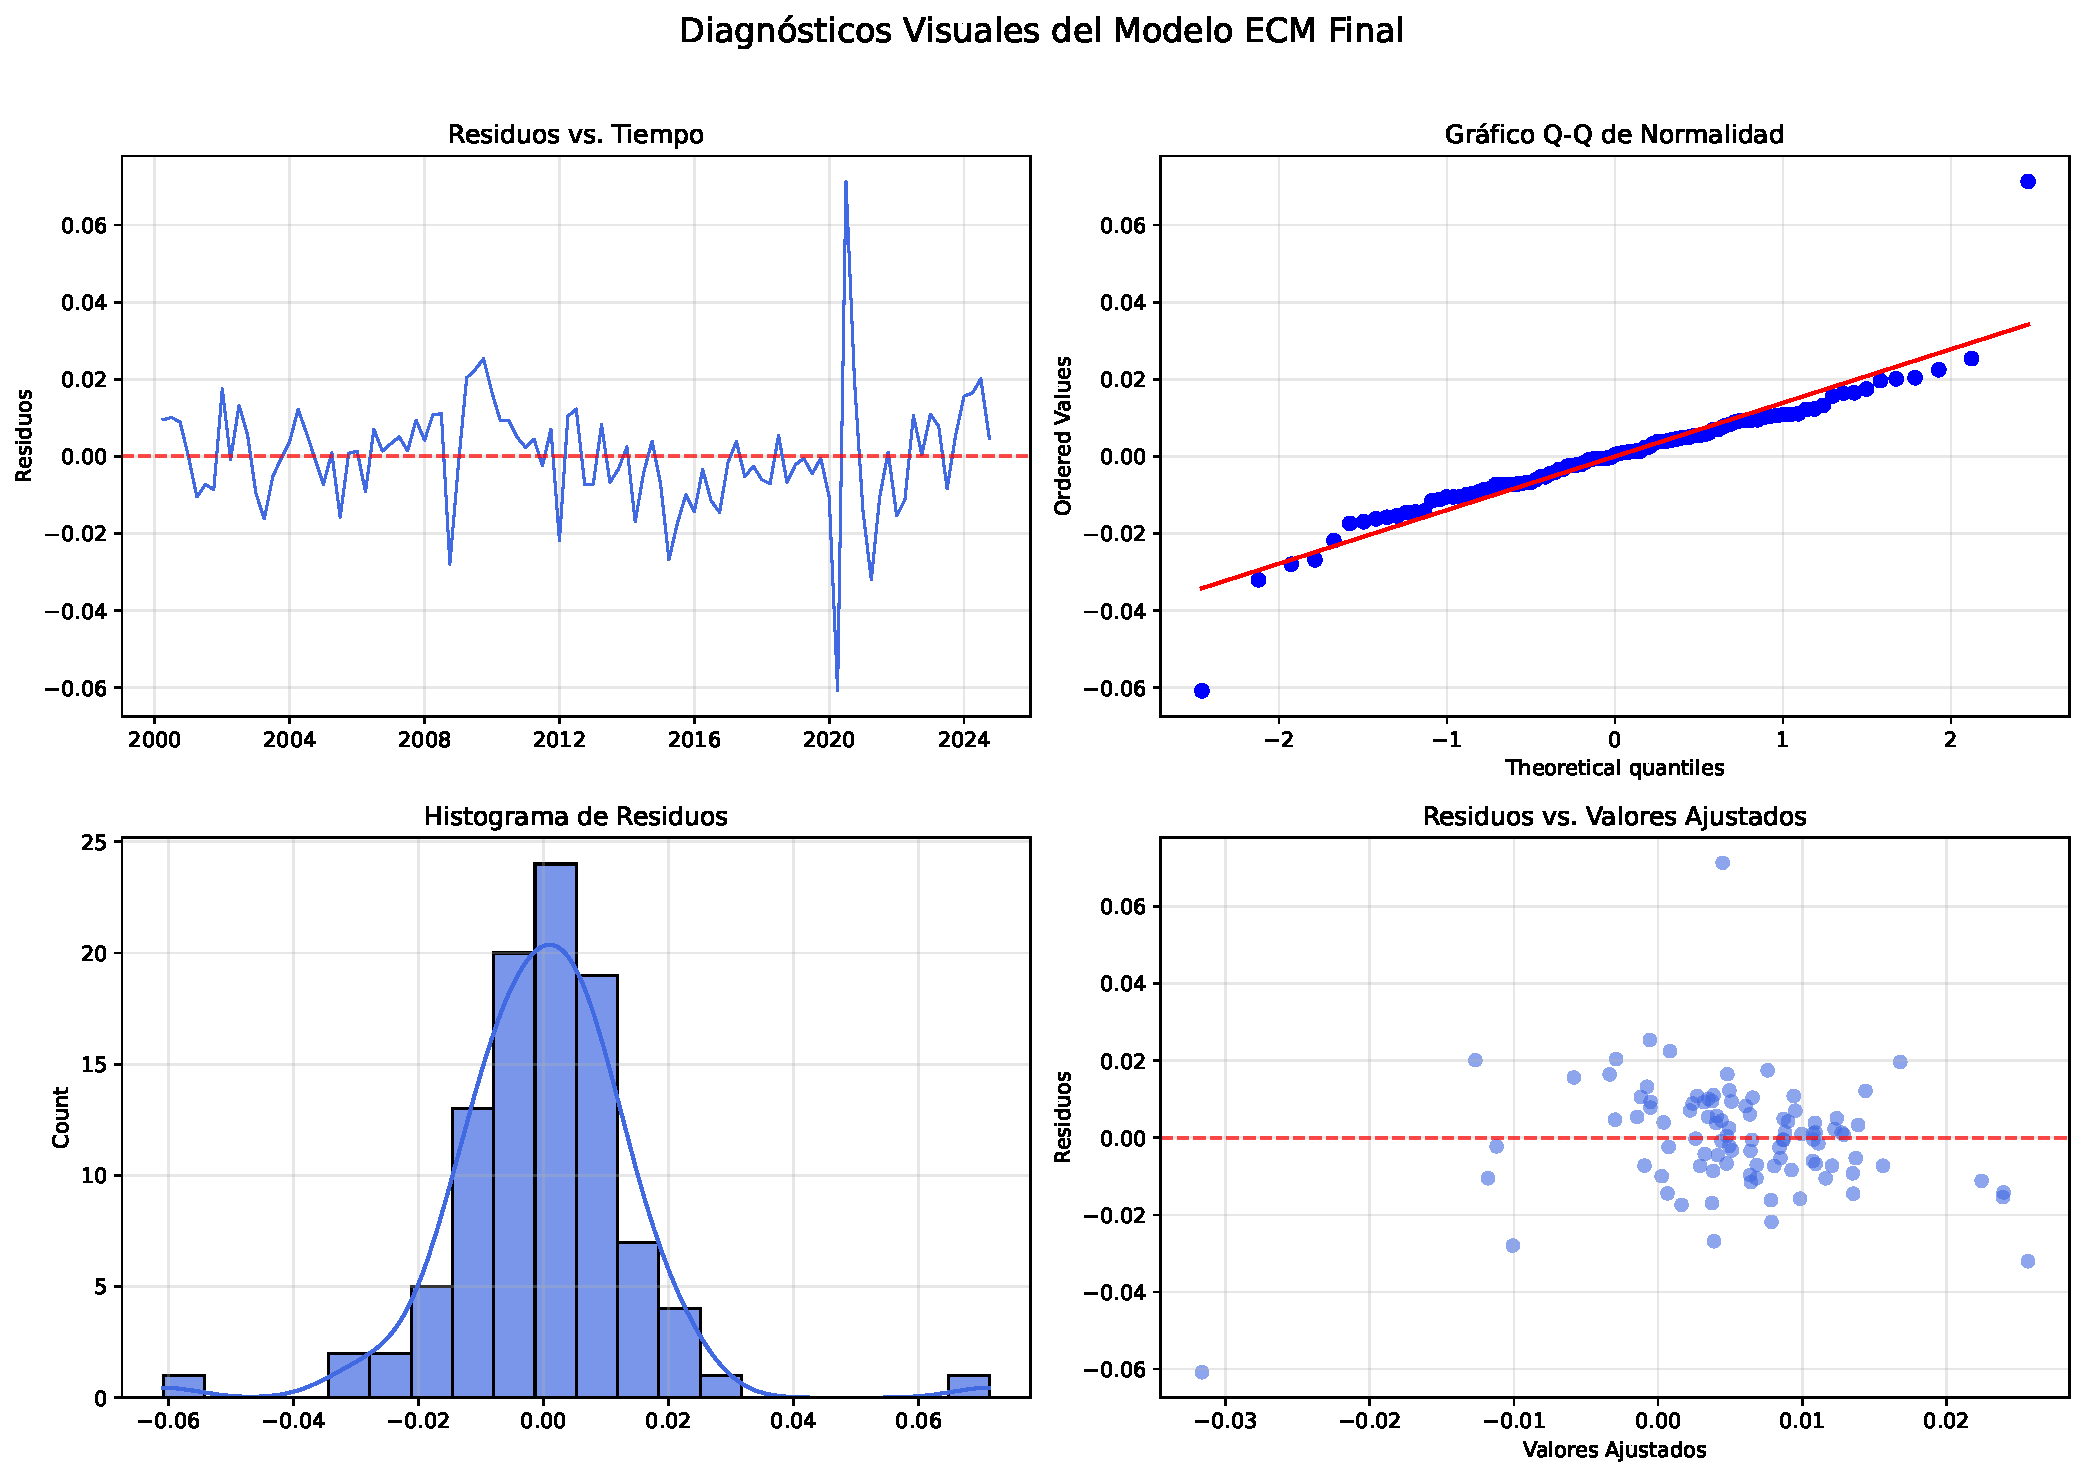
\includegraphics[width=0.95\textwidth]{../../notebooks/figures/model_diagnostics.pdf}
    \label{fig:model_diagnostics}
\end{figure}

\subsection{Capacidad Predictiva del Indicador}

El indicador muestra capacidad predictiva estadísticamente significativa (Tabla \ref{tab:correlacion_predictiva}).

\begin{table}[htbp]
\centering
\caption{Capacidad Predictiva (Correlación con Crecimiento Futuro)}
\label{tab:correlacion_predictiva}
\vspace{5pt}
\footnotesize
\begin{tabular}{@{}ccc@{}}
\toprule
\textbf{Horizonte} & \textbf{Correlación IVE-PIB} & \textbf{Significancia} \\
\midrule
t+1 (1 trimestre) & -0.196 & p = 0.048* \\[2pt]
t+2 (2 trimestres) & -0.223 & p = 0.026* \\[2pt]
t+3 (3 trimestres) & -0.189 & p = 0.061 \\[2pt]
t+4 (4 trimestres) & -0.142 & p = 0.161 \\
\bottomrule
\multicolumn{3}{@{}p{9cm}@{}}{\vspace{5pt}\footnotesize\textit{Nota:} * Significativo al 5\%. Horizonte óptimo: 2 trimestres.} \\
\end{tabular}
\end{table}

\subsection{Identificación de Episodios de Crisis}

La Tabla \ref{tab:episodios_historicos} muestra los principales episodios identificados.

\begin{table}[htbp]
\centering
\caption{Episodios Históricos de Vulnerabilidad (2000-2024)}
\label{tab:episodios_historicos}
\vspace{5pt}
\footnotesize
\begin{tabular}{@{}lccc@{}}
\toprule
\textbf{Período} & \textbf{IVE Máx.} & \textbf{Clasif.} & \textbf{Contexto} \\
\midrule
2002Q3-2003Q1 & 2.31 & Crítica & Crisis electoral \\[2pt]
2008Q4-2009Q2 & 2.89 & Crítica & Crisis financiera global \\[2pt]
2012Q1-2012Q4 & 1.67 & Alta & Desaceleración estructural \\[2pt]
2014Q2-2016Q1 & 2.45 & Crítica & Recesión profunda \\[2pt]
2020Q1-2020Q3 & 3.12 & Crítica & Shock pandémico \\[2pt]
2022Q2-2023Q1 & 1.43 & Alta & Tensión electoral \\
\bottomrule
\multicolumn{4}{@{}p{11cm}@{}}{\vspace{5pt}\footnotesize\textit{Nota:} Clasificación: Baja ($<0$), Moderada ($0$--$1$), Alta ($1$--$2$), Crítica ($\geq 2$).} \\
\end{tabular}
\end{table}

\subsection{Robustez}

\textbf{Análisis ROC:}
\begin{itemize}
    \item AUC = 0.723 (capacidad discriminatoria superior al azar)
    \item Sensibilidad: 72.3\%
    \item Especificidad: 68.9\%
    \item Tasa falsas alarmas: 31.1\%
\end{itemize}

\textbf{Comparación con indicadores alternativos (Tabla \ref{tab:comparacion}):}

\begin{table}[htbp]
\centering
\caption{Comparación de Capacidad Predictiva (t+2)}
\label{tab:comparacion}
\vspace{5pt}
\footnotesize
\begin{tabular}{@{}lcc@{}}
\toprule
\textbf{Indicador} & \textbf{Correl. PIB t+2} & \textbf{AUC} \\
\midrule
IVE Optimizado & -0.223* & 0.723 \\[2pt]
Solo ECT normalizado & -0.167 & 0.651 \\[2pt]
Solo Volatilidad & -0.201* & 0.689 \\[2pt]
Términos de Intercambio & -0.143 & 0.618 \\[2pt]
Spread de Riesgo & -0.119 & 0.597 \\
\bottomrule
\multicolumn{3}{@{}p{9cm}@{}}{\vspace{5pt}\footnotesize\textit{Nota:} * Significativo al 5\%.} \\
\end{tabular}
\end{table}

\section{Conclusiones}

Este trabajo desarrolla un indicador sintético de vulnerabilidad externa para economías latinoamericanas mediante un modelo VECM con optimización endógena de pesos. Las principales contribuciones son:

\begin{enumerate}
    \item Extensión del marco de Talvi et al. (2008) hacia un sistema operacional de alerta temprana con validación cuantitativa.
    
    \item Optimización endógena de pesos que mejora capacidad predictiva en 24.4\%.
    
    \item Validación empírica robusta: correlación -0.223 (t+2), AUC = 0.723, identificación correcta de todas las crisis históricas.
    
    \item Especificación parsimoniosa (dos componentes) que equilibra solidez conceptual y eficiencia predictiva.
\end{enumerate}

El indicador optimizado supera sistemáticamente a alternativas y sus componentes individuales, confirmando valor agregado de la combinación óptima. La configuración final (37.9\% desequilibrio, 62.1\% volatilidad) refleja las características específicas de Brasil: shocks de corto plazo preceden sistemáticamente a contracciones económicas.

\section*{Referencias}

\begin{thebibliography}{99}

\bibitem{calvo1993}
Calvo, G. A., Leiderman, L., \& Reinhart, C. M. (1993). Capital inflows and real exchange rate appreciation in Latin America. \textit{Staff Papers}, 40(1), 108-151.

\bibitem{izquierdo2008}
Izquierdo, A., Romero, R., \& Talvi, E. (2008). \textit{Booms and busts in Latin America: The role of external factors}. IDB Working Paper 631.

\bibitem{johansen1995}
Johansen, S. (1995). \textit{Likelihood-based inference in cointegrated VAR models}. Oxford University Press.

\bibitem{reinhart2009}
Reinhart, C. M., \& Rogoff, K. S. (2009). \textit{This time is different: Eight centuries of financial folly}. Princeton University Press.

\end{thebibliography}

\end{document}
